\documentclass[ignorenonframetext]{beamer}
\mode<presentation>
{
%\setbeamertemplate{background canvas}[vertical shading][bottom=red!10,top=blue!10]
%\usetheme[right]{PaloAlto}
%\usetheme{Warsaw}
\usetheme{Frankfurt}
%\usefonttheme[onlysmall]{structurebold}
%\usefonttheme{serif}
\usecolortheme{seahorse}
%\usecolortheme{rose}
%\usefonttheme[onlylarge]{structuresmallcapsserif}
%\usefonttheme[onlysmall]{structurebold}
%\setbeamerfont*{title}{shape=\itshape,family=\rmfamily}
\setbeamercolor{title}{fg=red!80!black}
%\setbeamercolor{title}{fg=red!80!black,bg=red!20!white}
%\setbeamercovered{transparent}
% % or whatever (possibly just delete it)
\setbeamercolor{math text}{fg=green!50!black}
%\setbeamercolor{normal text in math text}{parent=math text}
}
% -*- TeX:Rnw -*-
% ----------------------------------------------------------------
% .R Sweave file  ************************************************
% ----------------------------------------------------------------
%%
% \VignetteIndexEntry{}
% \VignetteDepends{}
% \VignettePackage{}
%\documentclass[a4paper,12pt]{article}
\usepackage[slovene]{babel}
\newcommand{\SVNRevision}{$ $Rev: 3 $ $}
%\newcommand{\SVNDate}{$ $Date:: 2009-02-2#$ $}
\newcommand{\SVNId}{$ $Id: program.Rnw 3 2009-02-22 17:36:08Z ABlejec $ $}
%\usepackage{babel}
%\input{abpkgB}
%\input{abpkg}
\input{abBeam}
\input{abcmd}
%\input{abpage}
\usepackage[cp1250]{inputenc}
\usepackage{pgf,pgfarrows,pgfnodes,pgfautomata,pgfheaps,pgfshade}
\usepackage{amsmath,amssymb}
\usepackage{colortbl}
\usepackage{Sweave}
\input{mysweaveB}
\newcommand{\BV}{}
\newcommand{\EV}{}
\newcommand{\myemph}[1]{{\color{Sgreen} \textit{#1}}}
\Sconcordance{concordance:analizaosebnih.tex:analizaosebnih.Rnw:%
1 60 1 1 6 1 1 1 8 1 2 4 0 1 2 11 1 1 2 21 0 %
1 3 4 1 1 2 110 0 1 2 5 1 1 2 15 0 1 4 1 1 1 %
2 16 0 1 4 13 1 1 2 20 0 1 2 5 1 1 2 20 0 1 %
2 6 1 1 2 6 0 1 3 11 1 1 2 17 0 1 5 8 1 1 2 %
4 0 2 2 4 0 1 2 7 1 1 2 7 0 1 3 9 1 1 2 15 0 %
1 5 1 1 1 2 8 0 1 4 9 1 1 2 12 0 1 2 4 1 1 2 %
94 0 1 2 5 1 1 2 20 0 1 2 5 1 1 2 20 0 1 2 9 %
1 1 2 1 3 8 1 1 2 1 3 4 1 1 2 4 0 1 2 6 1 1 %
2 1 4 5 1 1 2 9 0 1 3 5 1 1 2 23 0 1 5 7 1 1 %
2 48 0 1 11 6 1 1 2 1 10 5 1 1 2 14 0 1 4 10 %
1 1 2 20 0 1 6 5 1 1 2 15 0 1 5 6 1 1 2 30 0 %
1 8 5 1 1 2 1 10 7 1 1 2 1 5 6 1 1 2 22 0 1 %
4 7 1 1 2 48 0 1 11 6 1 1 2 1 10 5 1 1 2 14 %
0 1 4 10 1 1 2 20 0 1 6 5 1 1 2 15 0 1 5 6 1 %
1 2 30 0 1 8 5 1 1 2 1 10 5 1 1 2 1 19 5 1 1 %
2 1 19 6 1 1 2 11 0 1 2 10 1 1 2 21 0 1 4 5 %
1 1 2 11 0 1 4 4 1 1 2 25 0 1 4 4 1 1 2 34 0 %
1 8 5 1 1 2 11 0 1 2 7 1 1 2 8 0 1 3 2 1 1 2 %
8 0 1 3 5 1 1 2 1 10 11 1 1 2 1 3 5 1 1 2 8 %
0 1 7 5 1 1 2 49 0 1 9 8 1 1 2 1 7 6 1 1 2 %
34 0 1 5 5 1 1 2 1 9 5 1 1 2 21 0 1 2 7 1 1 %
2 1 9 6 1 1 2 1 9 6 1 1 2 1 9 8 1}

%\SweaveOpts{echo=false}
%\usepackage{lmodern}
%\input{abfont}
%\SweaveOpts{keep.source=true}
% ----------------------------------------------------------------
\title{Analiza podatko �tudentov biologije\\3. letnik 2011/12}
\author{Andrej Blejec}
%\address{}%
%\email{}%
%
%\thanks{}%
%\subjclass{}%
%\keywords{}%

%\date{}%
%\dedicatory{}%
%\commby{}%
\begin{document}
\mode<article> {\maketitle}
\mode<presentation> {\frame{\titlepage}}
\tableofcontents
% ----------------------------------------------------------------
\begin{abstract}
�tudentje biologije so v okviru predmeta Statistika pripravili zbirko podatkov o nekaterih telesnih merah sebe in star�ev.
V tem zapisu so prikazane nekatere mo�ne analize.
\end{abstract}
% -------------------------------------------------------------
%% Sweave settings for includegraphics default plot size (Sweave default is 0.8)
%% notice this must be after begin{document}
% \setkeys{Gin}{width=0.9\textwidth}
\setkeys{Gin}{width=0.7\textwidth}
% ----------------------------------------------------------------

\tableofcontents

\begin{Schunk}
\begin{Sinput}
> lfn <- "ST2011.txt"
\end{Sinput}
\end{Schunk}
Ime datoteke s podatki ST2011.txt.
% ----------------------------------------------------------------

\section{Vnos podatkov}

Podatki so bili zbrani na spletni strani predmeta \emph{BI022 Statistika} na sistemu
\href{http://pouk.bf.uni-lj.si/course/view.php?id=101}{Moodle}. Shranjeni so v datoteki
ST2011.txt.

%% |--------------------->>>>>>
\begin{frame}[fragile]
\frametitle{Vnos podatkov}
\begin{Schunk}
\begin{Sinput}
> data <- read.table(file.path("../data", 
+     lfn), sep = "\t", header = TRUE)
> str(data)
\end{Sinput}
\begin{Soutput}
'data.frame':	51 obs. of  12 variables:
 $ starost: int  58 23 21 20 21 20 21 21 21 23 ...
 $ mesec  : int  7 3 4 10 1 4 10 4 7 1 ...
 $ spol   : Factor w/ 2 levels "F �enski ","M mo�ki ": 2 1 1 1 1 1 1 1 1 2 ...
 $ masa   : int  88 54 42 60 52 56 58 77 60 95 ...
 $ visina : num  178 174 152 170 171 170 170 169 170 190 ...
 $ roke   : int  175 171 150 155 171 174 169 169 168 201 ...
 $ cevelj : int  44 40 37 39 39 40 39 40 39 46 ...
 $ lasje  : Factor w/ 2 levels "S svetli ","T temni ": 2 1 2 1 1 1 1 2 2 2 ...
 $ oci    : Factor w/ 2 levels "S svetli ","T temni ": 1 1 2 1 1 1 1 2 2 2 ...
 $ majica : Factor w/ 6 levels "L ","M ","S ",..: 1 3 6 2 2 3 2 2 3 4 ...
 $ mati   : num  150 173 157 160 173 174 155 170 155 174 ...
 $ oce    : int  180 189 159 190 183 186 179 175 189 176 ...
\end{Soutput}
\end{Schunk}
\end{frame}
%% <<<<<<---------------------|

Osnovni, vne�eni podatki

\begin{Schunk}
\begin{Sinput}
> data
\end{Sinput}
\begin{Soutput}
   starost mesec      spol masa visina roke
1       58     7  M mo�ki    88  178.0  175
2       23     3 F �enski    54  174.0  171
3       21     4 F �enski    42  152.0  150
4       20    10 F �enski    60  170.0  155
5       21     1 F �enski    52  171.0  171
6       20     4 F �enski    56  170.0  174
7       21    10 F �enski    58  170.0  169
8       21     4 F �enski    77  169.0  169
9       21     7 F �enski    60  170.0  168
10      23     1  M mo�ki    95  190.0  201
11      21     0  M mo�ki    73  173.0  179
12      22     9  M mo�ki    67  176.0  179
13      22     3 F �enski    58  173.0  172
14      22     9 F �enski    60  169.5  164
15      20     1 F �enski    55  164.0  168
16      20     9 F �enski    60  168.0  170
17      22     9  M mo�ki    63  177.0  185
18      20     3 F �enski    61  175.0  174
19      21     9 F �enski    61  166.0  175
20      21     8 F �enski    59  165.0  162
21      20    11 F �enski    55  162.0  160
22      20     4 F �enski    52  165.0    0
23      22     6 F �enski    62  167.0  165
24      21    12 F �enski    61  173.0  170
25      21     7 F �enski    55  158.0  155
26      22     0 F �enski    92  196.0    0
27      21     4 F �enski    57  171.0  166
28      23     2 F �enski    65  163.0  166
29      21     3  M mo�ki    57  168.0  168
30      21    11 F �enski    58  170.0  159
31      23     4  M mo�ki    83  179.0    0
32      22    10  M mo�ki    70  175.0  177
33      21     4 F �enski    60  170.0  167
34      21     5 F �enski    65  164.0    0
35      20     4 F �enski    56  172.0  171
36      22     5 F �enski    55  165.0  161
37      21     9 F �enski    66  164.0  166
38      21     6  M mo�ki    95  194.0  182
39      21     1 F �enski    58  163.0  160
40      21     6  M mo�ki    70  175.0  170
41      21     7 F �enski    55  170.0  171
42      22     7 F �enski    65  168.0  130
43      20    12 F �enski    64  172.0  156
44      20    11 F �enski    74  173.0  172
45      22     6 F �enski    57  161.0  150
46      21     2 F �enski    53  165.0  170
47      24     7  M mo�ki    66  178.0  176
48      20     1 F �enski    53  165.0  165
49      23     9 F �enski    62  166.0  166
50      22     9 F �enski    52  172.0  170
51      21     6 F �enski    49  164.0    8
   cevelj     lasje       oci majica  mati oce
1      44  T temni  S svetli      L  150.0 180
2      40 S svetli  S svetli      S  173.0 189
3      37  T temni   T temni    XXS  157.0 159
4      39 S svetli  S svetli      M  160.0 190
5      39 S svetli  S svetli      M  173.0 183
6      40 S svetli  S svetli      S  174.0 186
7      39 S svetli  S svetli      M  155.0 179
8      40  T temni   T temni      M  170.0 175
9      39  T temni   T temni      S  155.0 189
10     46  T temni   T temni     XL  174.0 176
11     43  T temni  S svetli      M  168.0 174
12     42 S svetli  S svetli      S  167.0 175
13     38  T temni   T temni      M  165.0 182
14     39 S svetli  S svetli      M  175.5 176
15     40  T temni  S svetli      S  158.0 183
16     40  T temni  S svetli      M  164.0 180
17     42 S svetli   T temni      M  155.0 177
18     41  T temni  S svetli      M  175.0 183
19     41  T temni   T temni      M  165.0 181
20     38  T temni   T temni      S  162.0 175
21     37 S svetli  S svetli      S  166.0 169
22     37  T temni   T temni      S  155.0 178
23     39  T temni  S svetli      S  166.0 168
24     39  T temni  S svetli      M  161.0 184
25     37  T temni   T temni      S  178.0 170
26     49  T temni   T temni      M    0.0   0
27     38  T temni   T temni      S  165.0   0
28     39  T temni  S svetli      M  161.0 176
29     41  T temni  S svetli      M  151.0 173
30     29 S svetli   T temni      S  160.0 179
31     43  T temni   T temni      M    0.0 177
32     43 S svetli  S svetli      L  158.0 179
33     39 S svetli  S svetli      S  169.0 177
34     40 S svetli  S svetli      M  168.0 182
35     40  T temni   T temni      S  163.0 181
36     38 S svetli  S svetli      S  170.0 180
37     40  T temni   T temni      M  172.0 184
38     43  T temni  S svetli      M  164.0 184
39     38  T temni   T temni      M  159.0 177
40     43  T temni   T temni      S  160.0 182
41     39 S svetli  S svetli     XS  173.0 181
42     39 S svetli  S svetli      S  164.0 184
43     38 S svetli   T temni      M  176.0 180
44     40  T temni   T temni      M  168.0 175
45     37  T temni   T temni      L   50.0  53
46     38  T temni  S svetli      M  160.0 172
47     42  T temni   T temni      M  170.0 175
48     39 S svetli  S svetli     XS  168.0 172
49     38  T temni   T temni      M  162.0 180
50     38  T temni  S svetli      S  175.0 180
51     38 S svetli  S svetli     XS  159.0 172
\end{Soutput}
\end{Schunk}


%% |--------------------->>>>>>
\begin{frame}[fragile]
\frametitle{Vrste spremenljivk}
Opisne spremenljivke
\begin{Schunk}
\begin{Sinput}
> opisne <- which(sapply(data, "class") == 
+     "factor")
> length(opisne)
\end{Sinput}
\begin{Soutput}
[1] 4
\end{Soutput}
\begin{Sinput}
> names(data)[opisne]
\end{Sinput}
\begin{Soutput}
[1] "spol"   "lasje"  "oci"    "majica"
\end{Soutput}
\end{Schunk}

�tevilske spremenljivke
\begin{Schunk}
\begin{Sinput}
> stevilske <- which(!sapply(data, "class") == 
+     "factor")
> length(stevilske)
\end{Sinput}
\begin{Soutput}
[1] 8
\end{Soutput}
\begin{Sinput}
> names(data)[stevilske]
\end{Sinput}
\begin{Soutput}
[1] "starost" "mesec"   "masa"    "visina" 
[5] "roke"    "cevelj"  "mati"    "oce"    
\end{Soutput}
\end{Schunk}
\end{frame}
%% <<<<<<---------------------|





\section{Pregled osnovnih podatkov }

Opisna statistika

%% |--------------------->>>>>>
\begin{frame}[fragile]
\frametitle{Opisna statistika}
\begin{Schunk}
\begin{Sinput}
> summary(data[, 1:6])
\end{Sinput}
\begin{Soutput}
    starost          mesec               spol   
 Min.   :20.00   Min.   : 0.000   F �enski :40  
 1st Qu.:21.00   1st Qu.: 3.500   M mo�ki  :11  
 Median :21.00   Median : 6.000                 
 Mean   :21.98   Mean   : 5.922                 
 3rd Qu.:22.00   3rd Qu.: 9.000                 
 Max.   :58.00   Max.   :12.000                 
      masa           visina           roke      
 Min.   :42.00   Min.   :152.0   Min.   :  0.0  
 1st Qu.:55.50   1st Qu.:165.0   1st Qu.:160.0  
 Median :60.00   Median :170.0   Median :168.0  
 Mean   :62.76   Mean   :170.4   Mean   :151.5  
 3rd Qu.:65.50   3rd Qu.:173.0   3rd Qu.:171.5  
 Max.   :95.00   Max.   :196.0   Max.   :201.0  
\end{Soutput}
\end{Schunk}
\end{frame}
%% <<<<<<---------------------|

%% |--------------------->>>>>>
\begin{frame}[fragile]
\frametitle{Opisna statistika}
\begin{Schunk}
\begin{Sinput}
> summary(data[, 7:12])
\end{Sinput}
\begin{Soutput}
     cevelj            lasje           oci    
 Min.   :29.00   S svetli :19   S svetli :28  
 1st Qu.:38.00   T temni  :32   T temni  :23  
 Median :39.00                                
 Mean   :39.71                                
 3rd Qu.:41.00                                
 Max.   :49.00                                
  majica        mati            oce       
 L   : 3   Min.   :  0.0   Min.   :  0.0  
 M   :25   1st Qu.:159.0   1st Qu.:175.0  
 S   :18   Median :164.0   Median :179.0  
 XL  : 1   Mean   :156.2   Mean   :168.9  
 XS  : 3   3rd Qu.:170.0   3rd Qu.:182.0  
 XXS : 1   Max.   :178.0   Max.   :190.0  
\end{Soutput}
\end{Schunk}
\end{frame}
%% <<<<<<---------------------|

Grafi�ni pregled podatkov
%% |--------------------->>>>>>
\begin{frame}[fragile]
\frametitle{Grafi�ni pregled podatkov}
\begin{Schunk}
\begin{Sinput}
> par(mfrow = c(3, 3))
> for (i in stevilske) plot(data[, i], main = names(data)[i])
\end{Sinput}
\end{Schunk}
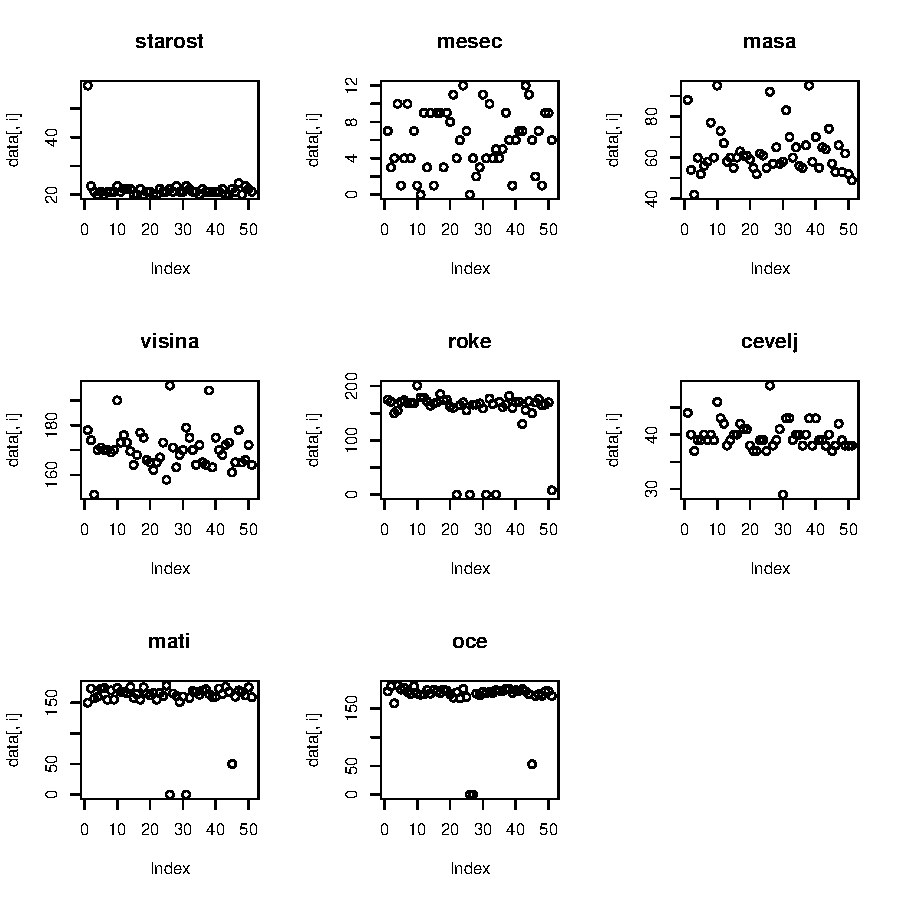
\includegraphics{./figs/SwPres-010}
\end{frame}
%% <<<<<<---------------------|


Pri zbiranju podatkov so manjkajo�e vrednosti spremenjene v vrednost ni�.  Za
nobeno spremenljivko taka vrednost ni smiselna, zato dobro ozna�uje
manjkajo�o vrednost. Zaradi enostavnej�e analize bomo enote s takimi
vrednostmi pri katerikoli spremenljivki izlo�ili.

%% |--------------------->>>>>>
\begin{frame}[fragile]
\frametitle{Odstranitev enot z manjkajo�imi podatki}
\begin{Schunk}
\begin{Sinput}
> nas <- which(apply(data, 1, function(x) any(as.numeric(x) == 
+     0)))
> nas
\end{Sinput}
\begin{Soutput}
[1] 11 22 26 27 31 34
\end{Soutput}
\begin{Sinput}
> if (length(nas) > 0) data <- data[-nas, 
+     ]
> dim(data)
\end{Sinput}
\begin{Soutput}
[1] 45 12
\end{Soutput}
\end{Schunk}
\end{frame}
%% <<<<<<---------------------|


Odstranimo �e podatke nenavadno starega �loveka in podatke osebe s kratko nogo.
%% |--------------------->>>>>>
\begin{frame}[fragile]
\frametitle{Odstranitev podatkov }
Odstranimo podatke prestarega �loveka :)
\begin{Schunk}
\begin{Sinput}
> data <- data[data$starost < 25, ]
\end{Sinput}
\end{Schunk}
in �e enega kratkorokega
\begin{Schunk}
\begin{Sinput}
> data <- data[data$roke > 50, ]
\end{Sinput}
\end{Schunk}
\end{frame}
%% <<<<<<---------------------|


Popravimo podatke
%% |--------------------->>>>>>
\begin{frame}[fragile]
\frametitle{Popravek podatkov}
\begin{Schunk}
\begin{Sinput}
> data[, "mati"] <- data[, "mati"] + 100 * 
+     (data[, "mati"] < 100)
> data[, "oce"] <- data[, "oce"] + 100 * 
+     (data[, "oce"] < 100)
\end{Sinput}
\end{Schunk}
\end{frame}
%% <<<<<<---------------------|

Pri prepisu podatkov iz sistema  Moodle dobijo vrednosti opisnih spremenljivk na koncu nepotreben znak presledek.
Odstranimo jih lahko z uporabo 'regularnih izrazov' (regular expression).

%% |--------------------->>>>>>
\begin{frame}[fragile]
\frametitle{Ureditev imen nivojev}
Odstranimo presledke v vrednostih
\begin{Schunk}
\begin{Sinput}
> x <- data[, "majica"]
> levels(x)
\end{Sinput}
\begin{Soutput}
[1] "L "   "M "   "S "   "XL "  "XS "  "XXS "
\end{Soutput}
\begin{Sinput}
> levels(x) <- gsub("(.*) ", "\\1", levels(x))
> levels(x)
\end{Sinput}
\begin{Soutput}
[1] "L"   "M"   "S"   "XL"  "XS"  "XXS"
\end{Soutput}
\end{Schunk}
\end{frame}
Neposredna sprememba imen nivojev
\begin{Schunk}
\begin{Sinput}
> levels(data[, "spol"]) <- c("zenski", 
+     "moski")
> levels(data[, "oci"]) <- c("svetle", "temne")
> levels(data[, "lasje"]) <- c("svetli", 
+     "temni")
\end{Sinput}
\end{Schunk}
%% <<<<<<---------------------|


Velikost majice je merjena na urejenostni lestvici, zato vrednosti uredimo po velikosti

%% |--------------------->>>>>>
\begin{frame}[fragile]
\frametitle{Urejenostna merska lestvica}

Spremenimo vrstni red nivojev
\begin{Schunk}
\begin{Sinput}
> (data[, "majica"] <- ordered(x, levels = c("XXS", 
+     "XS", "S", "M", "L", "XL")))
\end{Sinput}
\begin{Soutput}
 [1] S   XXS M   M   S   M   M   S   XL  S   M  
[12] M   S   M   M   M   M   S   S   S   M   S  
[23] M   M   S   L   S   S   S   M   M   M   S  
[34] XS  S   M   M   L   M   M   XS  M   S  
Levels: XXS < XS < S < M < L < XL
\end{Soutput}
\end{Schunk}
\end{frame}
%% <<<<<<---------------------|

\section{Pregled urejenih podatkov}

\begin{Schunk}
\begin{Sinput}
> data
\end{Sinput}
\begin{Soutput}
   starost mesec   spol masa visina roke cevelj
2       23     3 zenski   54  174.0  171     40
3       21     4 zenski   42  152.0  150     37
4       20    10 zenski   60  170.0  155     39
5       21     1 zenski   52  171.0  171     39
6       20     4 zenski   56  170.0  174     40
7       21    10 zenski   58  170.0  169     39
8       21     4 zenski   77  169.0  169     40
9       21     7 zenski   60  170.0  168     39
10      23     1  moski   95  190.0  201     46
12      22     9  moski   67  176.0  179     42
13      22     3 zenski   58  173.0  172     38
14      22     9 zenski   60  169.5  164     39
15      20     1 zenski   55  164.0  168     40
16      20     9 zenski   60  168.0  170     40
17      22     9  moski   63  177.0  185     42
18      20     3 zenski   61  175.0  174     41
19      21     9 zenski   61  166.0  175     41
20      21     8 zenski   59  165.0  162     38
21      20    11 zenski   55  162.0  160     37
23      22     6 zenski   62  167.0  165     39
24      21    12 zenski   61  173.0  170     39
25      21     7 zenski   55  158.0  155     37
28      23     2 zenski   65  163.0  166     39
29      21     3  moski   57  168.0  168     41
30      21    11 zenski   58  170.0  159     29
32      22    10  moski   70  175.0  177     43
33      21     4 zenski   60  170.0  167     39
35      20     4 zenski   56  172.0  171     40
36      22     5 zenski   55  165.0  161     38
37      21     9 zenski   66  164.0  166     40
38      21     6  moski   95  194.0  182     43
39      21     1 zenski   58  163.0  160     38
40      21     6  moski   70  175.0  170     43
41      21     7 zenski   55  170.0  171     39
42      22     7 zenski   65  168.0  130     39
43      20    12 zenski   64  172.0  156     38
44      20    11 zenski   74  173.0  172     40
45      22     6 zenski   57  161.0  150     37
46      21     2 zenski   53  165.0  170     38
47      24     7  moski   66  178.0  176     42
48      20     1 zenski   53  165.0  165     39
49      23     9 zenski   62  166.0  166     38
50      22     9 zenski   52  172.0  170     38
    lasje    oci majica  mati oce
2  svetli svetle      S 173.0 189
3   temni  temne    XXS 157.0 159
4  svetli svetle      M 160.0 190
5  svetli svetle      M 173.0 183
6  svetli svetle      S 174.0 186
7  svetli svetle      M 155.0 179
8   temni  temne      M 170.0 175
9   temni  temne      S 155.0 189
10  temni  temne     XL 174.0 176
12 svetli svetle      S 167.0 175
13  temni  temne      M 165.0 182
14 svetli svetle      M 175.5 176
15  temni svetle      S 158.0 183
16  temni svetle      M 164.0 180
17 svetli  temne      M 155.0 177
18  temni svetle      M 175.0 183
19  temni  temne      M 165.0 181
20  temni  temne      S 162.0 175
21 svetli svetle      S 166.0 169
23  temni svetle      S 166.0 168
24  temni svetle      M 161.0 184
25  temni  temne      S 178.0 170
28  temni svetle      M 161.0 176
29  temni svetle      M 151.0 173
30 svetli  temne      S 160.0 179
32 svetli svetle      L 158.0 179
33 svetli svetle      S 169.0 177
35  temni  temne      S 163.0 181
36 svetli svetle      S 170.0 180
37  temni  temne      M 172.0 184
38  temni svetle      M 164.0 184
39  temni  temne      M 159.0 177
40  temni  temne      S 160.0 182
41 svetli svetle     XS 173.0 181
42 svetli svetle      S 164.0 184
43 svetli  temne      M 176.0 180
44  temni  temne      M 168.0 175
45  temni  temne      L 150.0 153
46  temni svetle      M 160.0 172
47  temni  temne      M 170.0 175
48 svetli svetle     XS 168.0 172
49  temni  temne      M 162.0 180
50  temni svetle      S 175.0 180
\end{Soutput}
\end{Schunk}

\subsection{Opisna statistika}

%% |--------------------->>>>>>
\begin{frame}[fragile]
\frametitle{Opisna statistika}
\begin{Schunk}
\begin{Sinput}
> summary(data[, 1:6])
\end{Sinput}
\begin{Soutput}
    starost          mesec            spol   
 Min.   :20.00   Min.   : 1.000   zenski:35  
 1st Qu.:21.00   1st Qu.: 3.500   moski : 8  
 Median :21.00   Median : 7.000              
 Mean   :21.26   Mean   : 6.326              
 3rd Qu.:22.00   3rd Qu.: 9.000              
 Max.   :24.00   Max.   :12.000              
      masa           visina           roke      
 Min.   :42.00   Min.   :152.0   Min.   :130.0  
 1st Qu.:55.50   1st Qu.:165.0   1st Qu.:163.0  
 Median :60.00   Median :170.0   Median :169.0  
 Mean   :61.44   Mean   :169.7   Mean   :167.4  
 3rd Qu.:64.50   3rd Qu.:173.0   3rd Qu.:171.5  
 Max.   :95.00   Max.   :194.0   Max.   :201.0  
\end{Soutput}
\end{Schunk}
\end{frame}
%% <<<<<<---------------------|

%% |--------------------->>>>>>
\begin{frame}[fragile]
\frametitle{Opisna statistika}
\begin{Schunk}
\begin{Sinput}
> summary(data[, 7:12])
\end{Sinput}
\begin{Soutput}
     cevelj         lasje        oci     majica  
 Min.   :29.00   svetli:17   svetle:24   XXS: 1  
 1st Qu.:38.00   temni :26   temne :19   XS : 2  
 Median :39.00                           S  :16  
 Mean   :39.37                           M  :21  
 3rd Qu.:40.00                           L  : 2  
 Max.   :46.00                           XL : 1  
      mati            oce       
 Min.   :150.0   Min.   :153.0  
 1st Qu.:160.0   1st Qu.:175.0  
 Median :165.0   Median :179.0  
 Mean   :165.2   Mean   :178.0  
 3rd Qu.:171.0   3rd Qu.:182.5  
 Max.   :178.0   Max.   :190.0  
\end{Soutput}
\end{Schunk}
\end{frame}
%% <<<<<<---------------------|

\subsection{Porazdelitve podatkov}

Porazdelitve opisnih spremenljivk

%% |--------------------->>>>>>
\begin{frame}[fragile]
\frametitle{Porazdelitve opisnih spremenljivk}
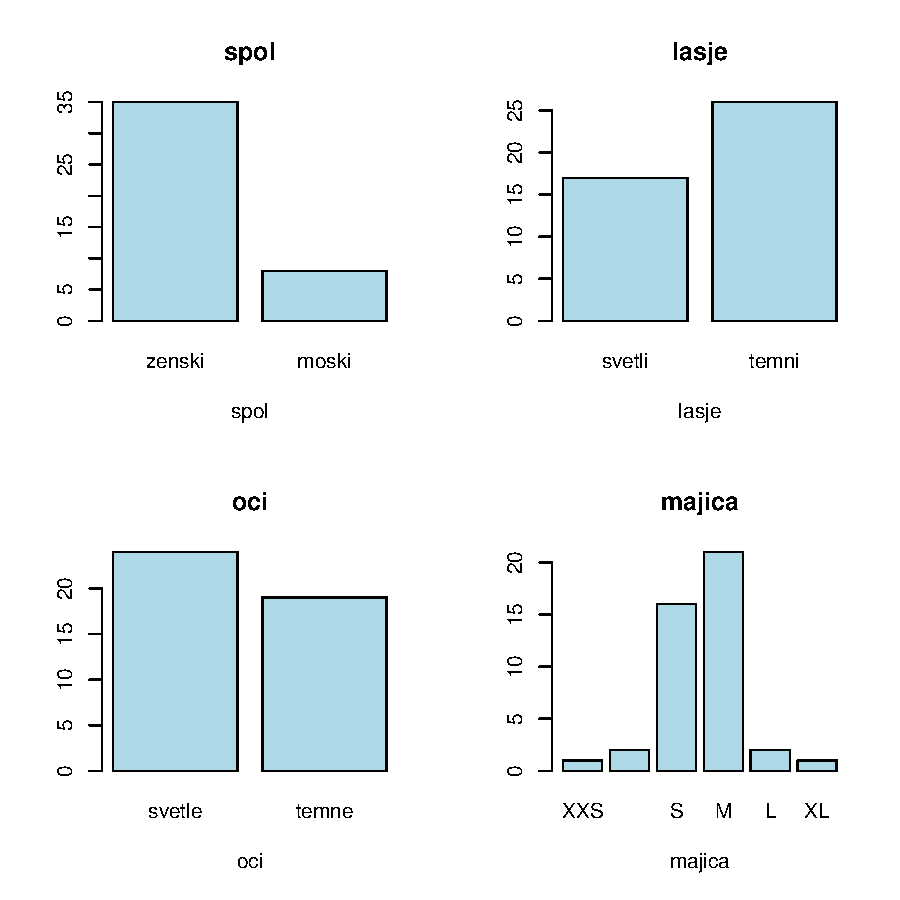
\includegraphics{./figs/SwPres-021}
\end{frame}
%% <<<<<<---------------------|


Porazdelitve �tevilskih spremenljivk

%% |--------------------->>>>>>
\begin{frame}[fragile]
\frametitle{Porazdelitve �tevilskih spremenljivk}
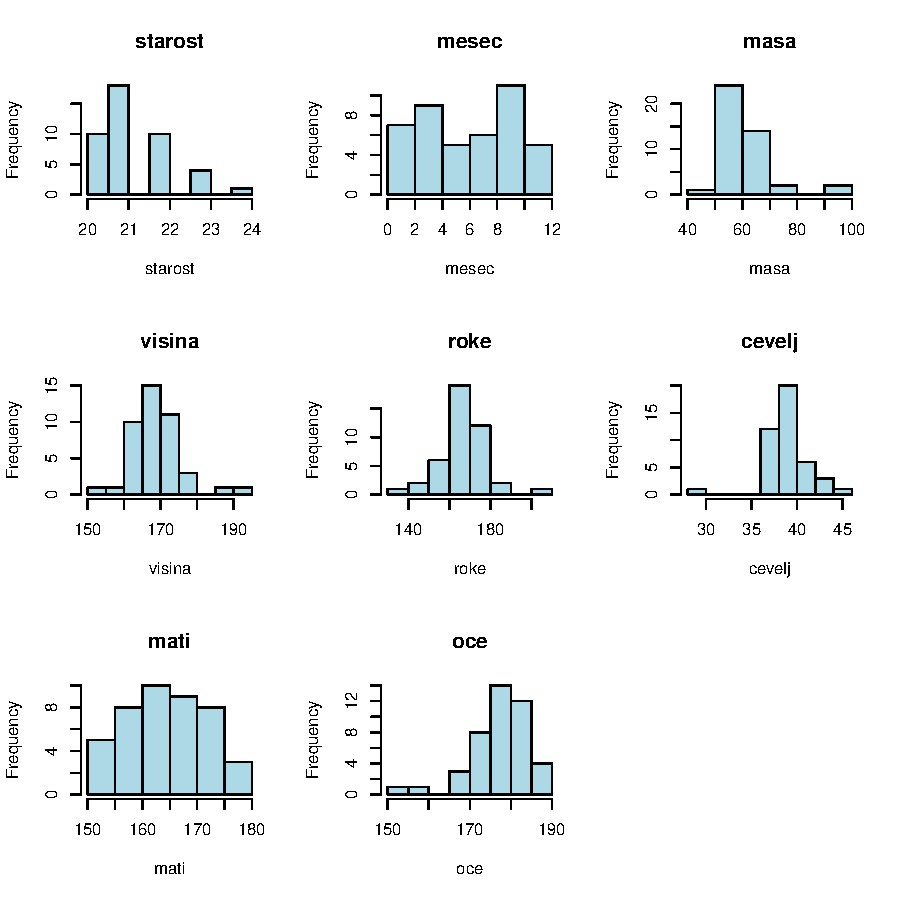
\includegraphics{./figs/SwPres-022}
\end{frame}
%% <<<<<<---------------------|

Omogo�imo neposredno rabo spremenljivk.

\begin{Schunk}
\begin{Sinput}
> attach(data)
\end{Sinput}
\end{Schunk}
\clearpage
\section{Testiranje hipotez}

\subsection{Ali so fantje ve�ji od deklet?}
%% |--------------------->>>>>>
\begin{frame}[fragile]
\frametitle{Porazdelitvi}
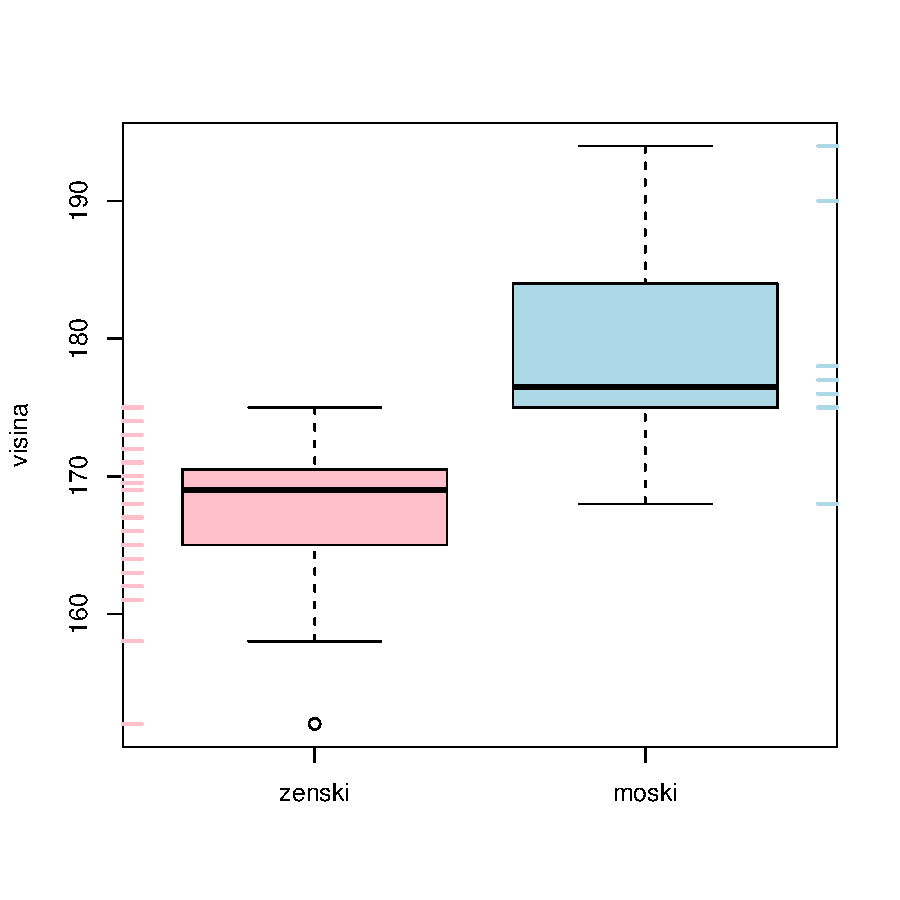
\includegraphics{./figs/SwPres-boxvis}
\end{frame}
%% <<<<<<---------------------|

%% |--------------------->>>>>>
\begin{frame}[fragile]
\frametitle{Porazdelitvi - R ukazi}
\begin{Schunk}
\begin{Sinput}
> boxplot(visina ~ spol, col = c("pink", 
+     "lightblue"), ylab = "visina")
> rug(visina[spol == "zenski"], side = 2, 
+     col = "pink", lwd = 2)
> rug(visina[!spol == "zenski"], side = 4, 
+     , col = "lightblue", lwd = 2)
\end{Sinput}
\end{Schunk}
\end{frame}
%% <<<<<<---------------------|

%% |--------------------->>>>>>
\begin{frame}[fragile]
\frametitle{Opisni pregled}
\begin{Schunk}
\begin{Sinput}
> y <- visina
> (n <- tapply(y, spol, length))
\end{Sinput}
\begin{Soutput}
zenski  moski 
    35      8 
\end{Soutput}
\begin{Sinput}
> (xbar <- tapply(y, spol, mean))
\end{Sinput}
\begin{Soutput}
  zenski    moski 
167.5857 179.1250 
\end{Soutput}
\begin{Sinput}
> (s <- tapply(y, spol, sd))
\end{Sinput}
\begin{Soutput}
  zenski    moski 
4.881667 8.559665 
\end{Soutput}
\end{Schunk}
\end{frame}
%% <<<<<<---------------------|



%% |--------------------->>>>>>
\begin{frame}[fragile]
\frametitle{Ali sta varianci zna�ilno razli�ni?}
\begin{Schunk}
\begin{Sinput}
> alpha <- 0.01
> (v <- sort(s^2))
\end{Sinput}
\begin{Soutput}
  zenski    moski 
23.83067 73.26786 
\end{Soutput}
\begin{Sinput}
> ns <- as.vector(n[order(s)])
> (F <- as.vector(v[2]/v[1]))
\end{Sinput}
\begin{Soutput}
[1] 3.074519
\end{Soutput}
\begin{Sinput}
> (df1 <- ns[2] - 1)
\end{Sinput}
\begin{Soutput}
[1] 7
\end{Soutput}
\begin{Sinput}
> (df2 <- ns[1] - 1)
\end{Sinput}
\begin{Soutput}
[1] 34
\end{Soutput}
\begin{Sinput}
> (F.krit <- qf(1 - alpha, df1, df2))
\end{Sinput}
\begin{Soutput}
[1] 3.218154
\end{Soutput}
\begin{Sinput}
> (p <- 1 - pf(F, df1, df2))
\end{Sinput}
\begin{Soutput}
[1] 0.01278561
\end{Soutput}
\begin{Sinput}
> if (F < F.krit) cat("Varianci NISTA statisti�no zna�ilno razli�ni (p =", 
+     round(p, 3), ").\n") else cat("Varianci STA  statisti�no zan�ilno razli�ni (p <", 
+     alpha, ") (p =", round(p, 3), ").\n")
\end{Sinput}
\begin{Soutput}
Varianci NISTA statisti�no zna�ilno razli�ni (p = 0.013 ).
\end{Soutput}
\end{Schunk}

\end{frame}
%% <<<<<<---------------------|

%% |--------------------->>>>>>
\begin{frame}[fragile]
\frametitle{Ali sta varianci zna�ilno razli�ni?}
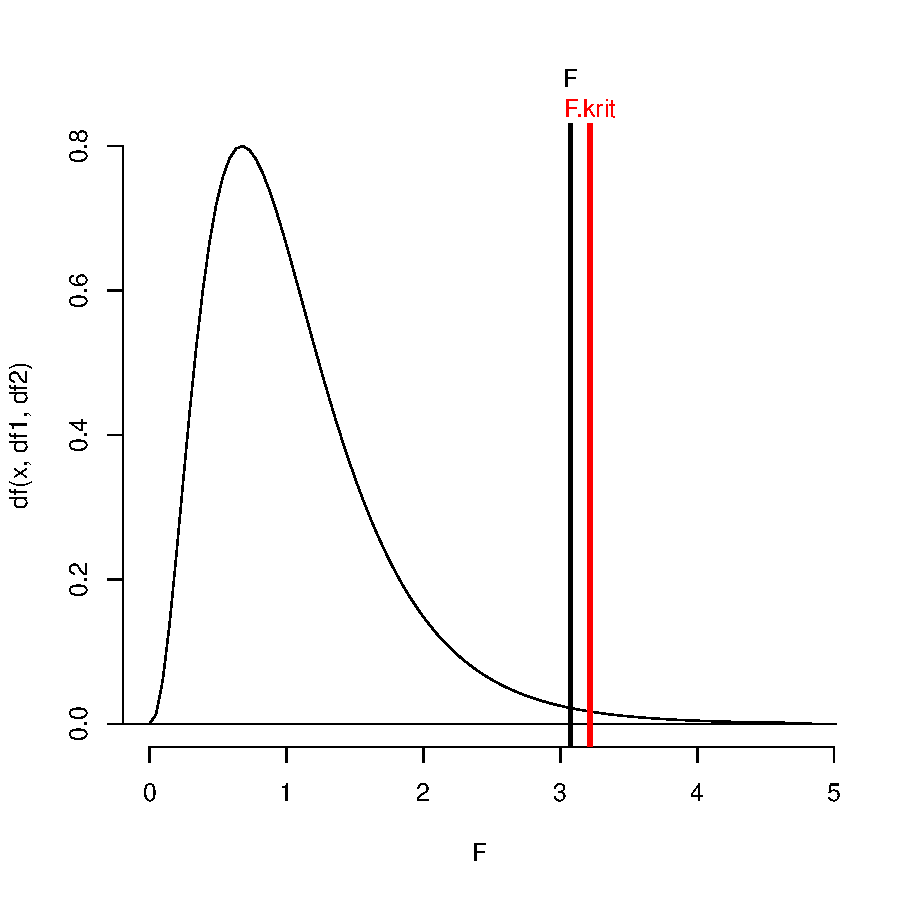
\includegraphics{./figs/SwPres-critvisF}
\end{frame}
%% <<<<<<---------------------|

%% |--------------------->>>>>>
\begin{frame}[fragile]
\frametitle{Kako smo narisali sliko?}
\begin{Schunk}
\begin{Sinput}
> x <- seq(0, max(F, F.krit) * 1.5, length = 100)
> plot(x, df(x, df1, df2), type = "l", xlab = "F", 
+     axes = FALSE)
> axis(1)
> axis(2)
> abline(h = 0)
> abline(v = F, lwd = 3)
> mtext("F", side = 3, line = 1, at = F)
> abline(v = F.krit, col = "red", lwd = 3)
> mtext("F.krit", side = 3, line = 0, at = F.krit, 
+     col = "red")
\end{Sinput}
\end{Schunk}
\end{frame}
%% <<<<<<---------------------|

Studentov t-test razlike povpre�ij

%% |--------------------->>>>>>
\begin{frame}[fragile]
\frametitle{Hipoteze in delni rezultati}
Uredimo vrstni red delnih rezultatov za test hipotez
$$H_0: \mu_{moski}=\mu_{zenski}+\Delta$$
$$H_1: \mu_{moski}>\mu_{zenski}+\Delta$$
\begin{Schunk}
\begin{Sinput}
> ord <- c("moski", "zenski")
> (xbar <- as.vector(xbar[ord]))
\end{Sinput}
\begin{Soutput}
[1] 179.1250 167.5857
\end{Soutput}
\begin{Sinput}
> (s <- as.vector(s[ord]))
\end{Sinput}
\begin{Soutput}
[1] 8.559665 4.881667
\end{Soutput}
\begin{Sinput}
> (n <- as.vector(n[ord]))
\end{Sinput}
\begin{Soutput}
[1]  8 35
\end{Soutput}
\end{Schunk}
\end{frame}
%% <<<<<<---------------------|

%% |--------------------->>>>>>
\begin{frame}[fragile]
\frametitle{Stopnja tveganja in kriti�ne vrednosti}
\begin{Schunk}
\begin{Sinput}
> alpha <- 0.01
> delta <- 0
> (df <- n[1] + n[2] - 2)
\end{Sinput}
\begin{Soutput}
[1] 41
\end{Soutput}
\begin{Sinput}
> (t.krit <- qt(1 - alpha, df))
\end{Sinput}
\begin{Soutput}
[1] 2.420803
\end{Soutput}
\end{Schunk}
\end{frame}
%% <<<<<<---------------------|


%% |--------------------->>>>>>
\begin{frame}[fragile]
\frametitle{Studentov t-test}
\begin{Schunk}
\begin{Sinput}
> xbar[1] - xbar[2]
\end{Sinput}
\begin{Soutput}
[1] 11.53929
\end{Soutput}
\begin{Sinput}
> s2 <- ((n[1] - 1) * s[1]^2 + (n[2] - 1) * 
+     s[2]^2)/(n[1] + n[2] - 2)
> (t <- (xbar[1] - xbar[2] - delta)/sqrt(s2) * 
+     sqrt(n[1] * n[2]/(n[1] + n[2])))
\end{Sinput}
\begin{Soutput}
[1] 5.18342
\end{Soutput}
\begin{Sinput}
> (p <- 1 - pt(t, df))
\end{Sinput}
\begin{Soutput}
[1] 3.102809e-06
\end{Soutput}
\begin{Sinput}
> if (t < t.krit) cat("Povpre�je1 NI statisti�no zna�ilno ve�je (p =", 
+     round(p, 3), ").\n") else cat("Povpre�je1 JE  statisti�no zan�ilno ve�je (p <", 
+     alpha, ") (p =", round(p, 3), ").\n")
\end{Sinput}
\begin{Soutput}
Povpre�je1 JE  statisti�no zan�ilno ve�je (p < 0.01 ) (p = 0 ).
\end{Soutput}
\end{Schunk}
\end{frame}
%% <<<<<<---------------------|

%% |--------------------->>>>>>
\begin{frame}[fragile]
\frametitle{Slika}
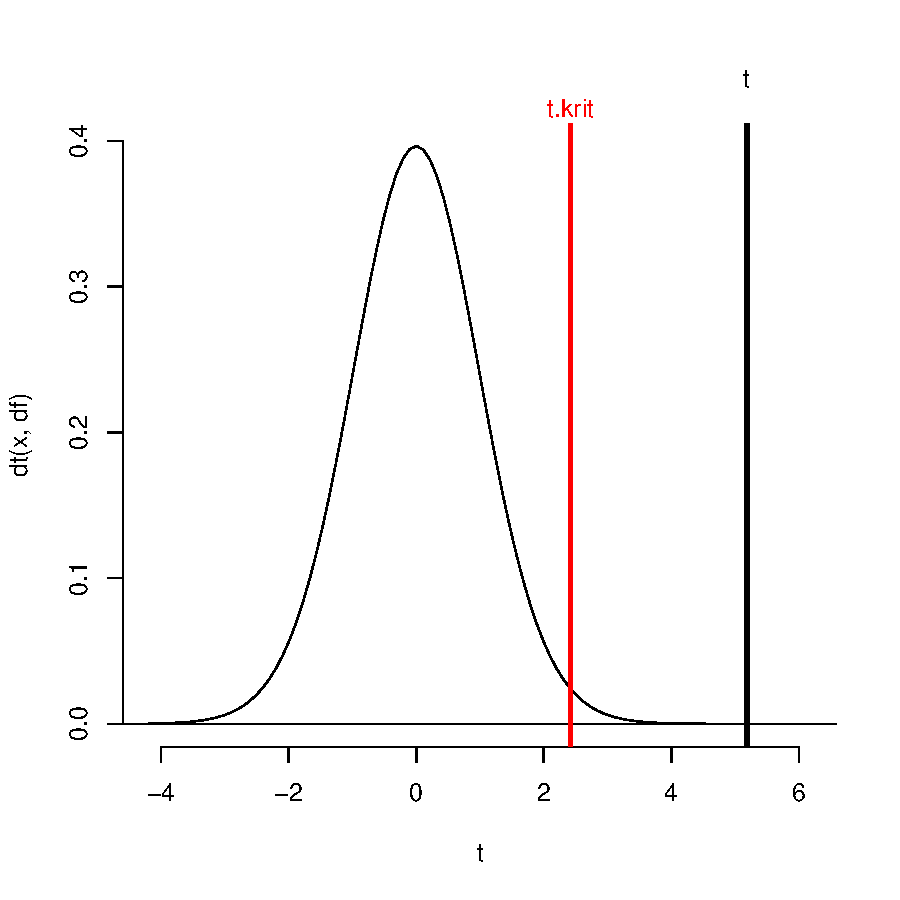
\includegraphics{./figs/SwPres-critvist}
\end{frame}
%% <<<<<<---------------------|

\subsection{Ali so fantje tezji od deklet?}

%% |--------------------->>>>>>
\begin{frame}[fragile]
\frametitle{Porazdelitvi}
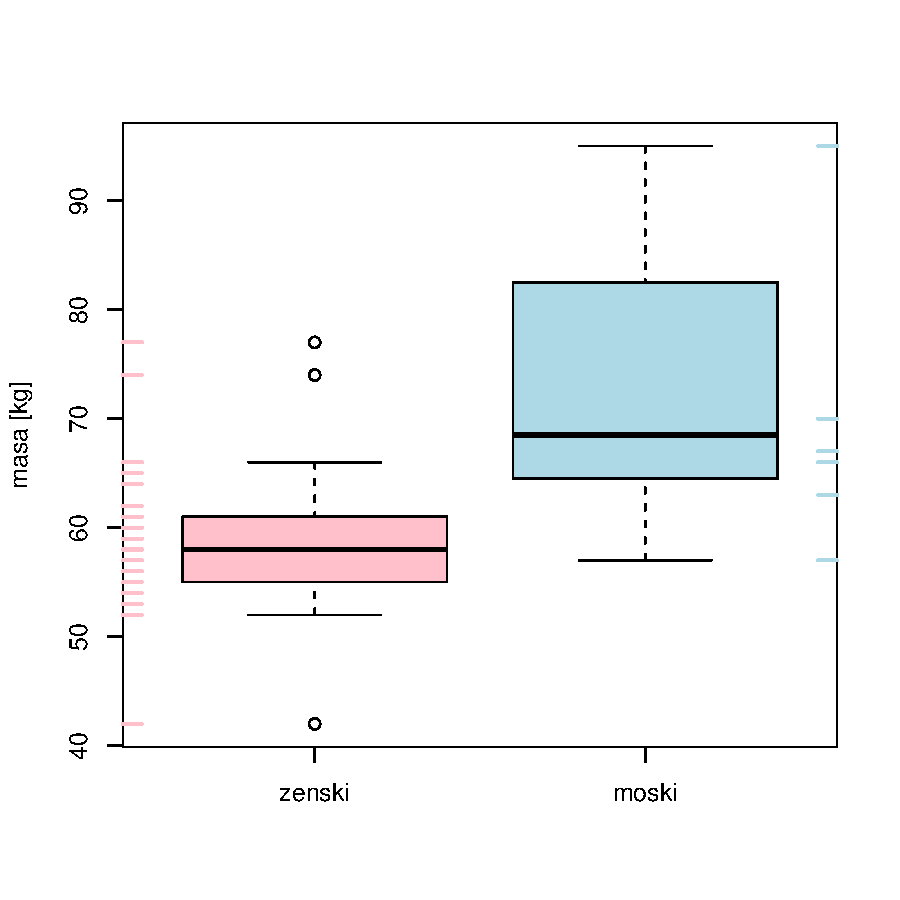
\includegraphics{./figs/SwPres-034}
\end{frame}
%% <<<<<<---------------------|


%% |--------------------->>>>>>
\begin{frame}[fragile]
\frametitle{Opisni pregled}
\begin{Schunk}
\begin{Sinput}
> (n <- tapply(y, spol, length))
\end{Sinput}
\begin{Soutput}
zenski  moski 
    35      8 
\end{Soutput}
\begin{Sinput}
> (xbar <- tapply(y, spol, mean))
\end{Sinput}
\begin{Soutput}
  zenski    moski 
58.82857 72.87500 
\end{Soutput}
\begin{Sinput}
> (s <- tapply(y, spol, sd))
\end{Sinput}
\begin{Soutput}
   zenski     moski 
 6.228425 14.277230 
\end{Soutput}
\end{Schunk}
\end{frame}
%% <<<<<<---------------------|



%% |--------------------->>>>>>
\begin{frame}[fragile]
\frametitle{Ali sta varianci zna�ilno razli�ni?}
\begin{Schunk}
\begin{Sinput}
> alpha <- 0.01
> (v <- sort(s^2))
\end{Sinput}
\begin{Soutput}
   zenski     moski 
 38.79328 203.83929 
\end{Soutput}
\begin{Sinput}
> ns <- as.vector(n[order(s)])
> (F <- as.vector(v[2]/v[1]))
\end{Sinput}
\begin{Soutput}
[1] 5.2545
\end{Soutput}
\begin{Sinput}
> (df1 <- ns[2] - 1)
\end{Sinput}
\begin{Soutput}
[1] 7
\end{Soutput}
\begin{Sinput}
> (df2 <- ns[1] - 1)
\end{Sinput}
\begin{Soutput}
[1] 34
\end{Soutput}
\begin{Sinput}
> (F.krit <- qf(1 - alpha, df1, df2))
\end{Sinput}
\begin{Soutput}
[1] 3.218154
\end{Soutput}
\begin{Sinput}
> (p <- 1 - pf(F, df1, df2))
\end{Sinput}
\begin{Soutput}
[1] 0.0003909851
\end{Soutput}
\begin{Sinput}
> if (F < F.krit) cat("Varianci NISTA statisti�no zna�ilno razli�ni (p =", 
+     round(p, 3), ").\n") else cat("Varianci STA  statisti�no zan�ilno razli�ni (p <", 
+     alpha, ") (p =", round(p, 3), ").\n")
\end{Sinput}
\begin{Soutput}
Varianci STA  statisti�no zan�ilno razli�ni (p < 0.01 ) (p = 0 ).
\end{Soutput}
\end{Schunk}

\end{frame}
%% <<<<<<---------------------|

%% |--------------------->>>>>>
\begin{frame}[fragile]
\frametitle{Ali sta varianci zna�ilno razli�ni?}
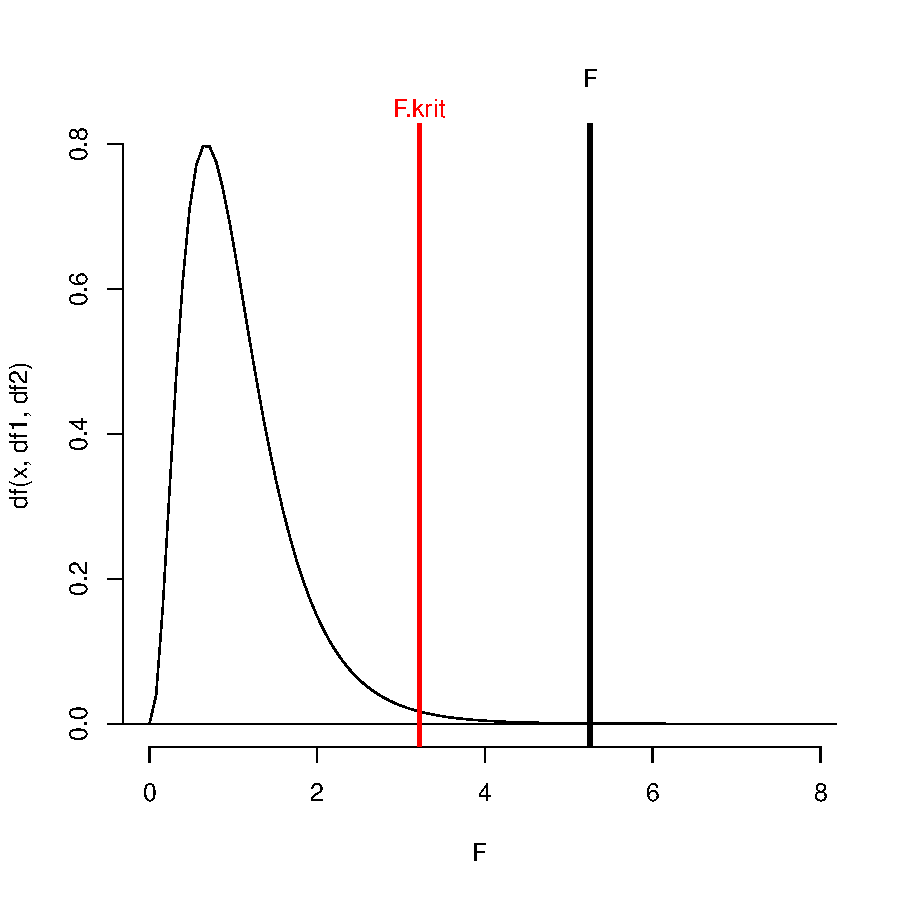
\includegraphics{./figs/SwPres-crittezaF}
\end{frame}
%% <<<<<<---------------------|

%% |--------------------->>>>>>
\begin{frame}[fragile]
\frametitle{Kako smo narisali sliko?}
\begin{Schunk}
\begin{Sinput}
> x <- seq(0, max(F, F.krit) * 1.5, length = 100)
> plot(x, df(x, df1, df2), type = "l", xlab = "F", 
+     axes = FALSE)
> axis(1)
> axis(2)
> abline(h = 0)
> abline(v = F, lwd = 3)
> mtext("F", side = 3, line = 1, at = F)
> abline(v = F.krit, col = "red", lwd = 3)
> mtext("F.krit", side = 3, line = 0, at = F.krit, 
+     col = "red")
\end{Sinput}
\end{Schunk}
\end{frame}
%% <<<<<<---------------------|

Studentov t-test razlike povpre�ij

%% |--------------------->>>>>>
\begin{frame}[fragile]
\frametitle{Hipoteze in delni rezultati}
Uredimo vrstni red delnih rezultatov za test hipotez
$$H_0: \mu_{moski}=\mu_{zenski}+\delta$$
$$H_1: \mu_{moski}>\mu_{zenski}+\delta$$
\begin{Schunk}
\begin{Sinput}
> ord <- c("moski", "zenski")
> (xbar <- as.vector(xbar[ord]))
\end{Sinput}
\begin{Soutput}
[1] 72.87500 58.82857
\end{Soutput}
\begin{Sinput}
> (s <- as.vector(s[ord]))
\end{Sinput}
\begin{Soutput}
[1] 14.277230  6.228425
\end{Soutput}
\begin{Sinput}
> (n <- as.vector(n[ord]))
\end{Sinput}
\begin{Soutput}
[1]  8 35
\end{Soutput}
\end{Schunk}
\end{frame}
%% <<<<<<---------------------|

%% |--------------------->>>>>>
\begin{frame}[fragile]
\frametitle{Stopnja tveganja in kriti�ne vrednosti}
\begin{Schunk}
\begin{Sinput}
> alpha <- 0.01
> delta <- 0
> (df <- n[1] + n[2] - 2)
\end{Sinput}
\begin{Soutput}
[1] 41
\end{Soutput}
\begin{Sinput}
> (t.krit <- qt(1 - alpha, df))
\end{Sinput}
\begin{Soutput}
[1] 2.420803
\end{Soutput}
\end{Schunk}
\end{frame}
%% <<<<<<---------------------|


%% |--------------------->>>>>>
\begin{frame}[fragile]
\frametitle{Studentov t-test}
\begin{Schunk}
\begin{Sinput}
> xbar[1] - xbar[2]
\end{Sinput}
\begin{Soutput}
[1] 14.04643
\end{Soutput}
\begin{Sinput}
> s2 <- ((n[1] - 1) * s[1]^2 + (n[2] - 1) * 
+     s[2]^2)/(n[1] + n[2] - 2)
> (t <- (xbar[1] - xbar[2] - delta)/sqrt(s2) * 
+     sqrt(n[1] * n[2]/(n[1] + n[2])))
\end{Sinput}
\begin{Soutput}
[1] 4.379903
\end{Soutput}
\begin{Sinput}
> (p <- 1 - pt(t, df))
\end{Sinput}
\begin{Soutput}
[1] 4.012688e-05
\end{Soutput}
\begin{Sinput}
> if (t < t.krit) cat("Povpre�je1 NI statisti�no zna�ilno ve�je (p =", 
+     round(p, 3), ").\n") else cat("Povpre�je1 JE  statisti�no zan�ilno ve�je (p <", 
+     alpha, ") (p =", round(p, 3), ").\n")
\end{Sinput}
\begin{Soutput}
Povpre�je1 JE  statisti�no zan�ilno ve�je (p < 0.01 ) (p = 0 ).
\end{Soutput}
\end{Schunk}
\end{frame}
%% <<<<<<---------------------|

%% |--------------------->>>>>>
\begin{frame}[fragile]
\frametitle{Slika}
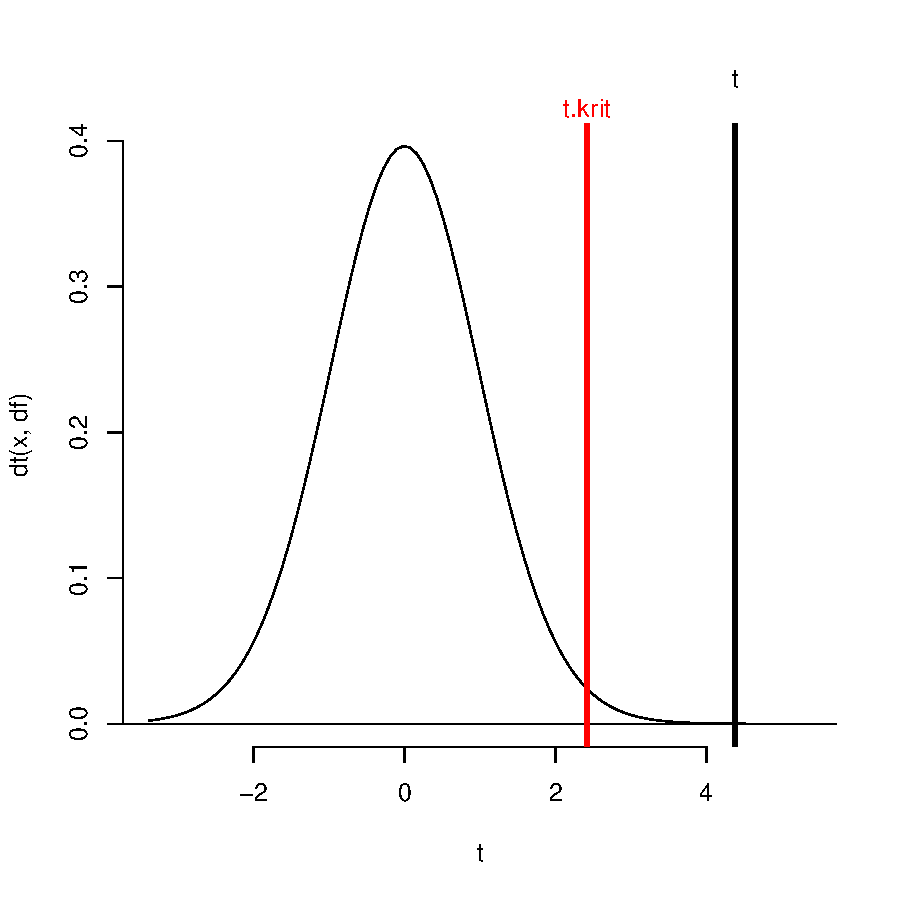
\includegraphics{./figs/SwPres-042}
\end{frame}
%% <<<<<<---------------------|

%% |--------------------->>>>>>
\begin{frame}[fragile]
\frametitle{Neparametri�ni test - Wilcoxon}
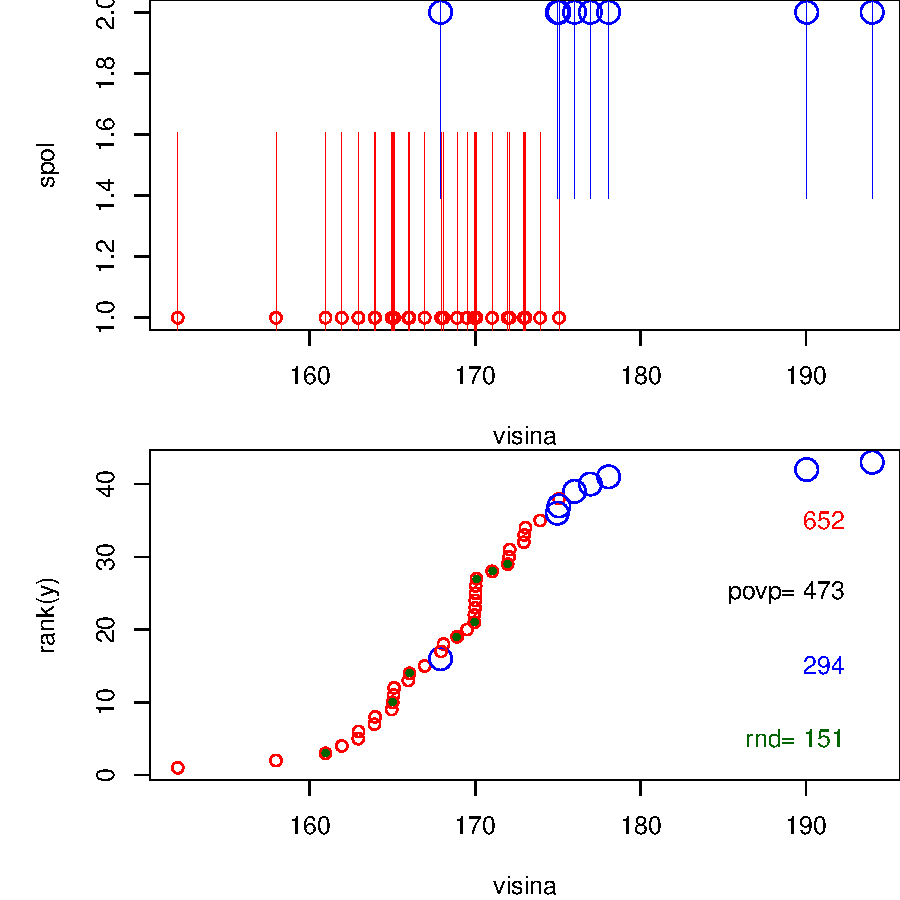
\includegraphics{./figs/SwPres-043}
\end{frame}
%% <<<<<<---------------------|

%% |--------------------->>>>>>
\begin{frame}[fragile]
\frametitle{Randomizacijski test - vsota rangov}
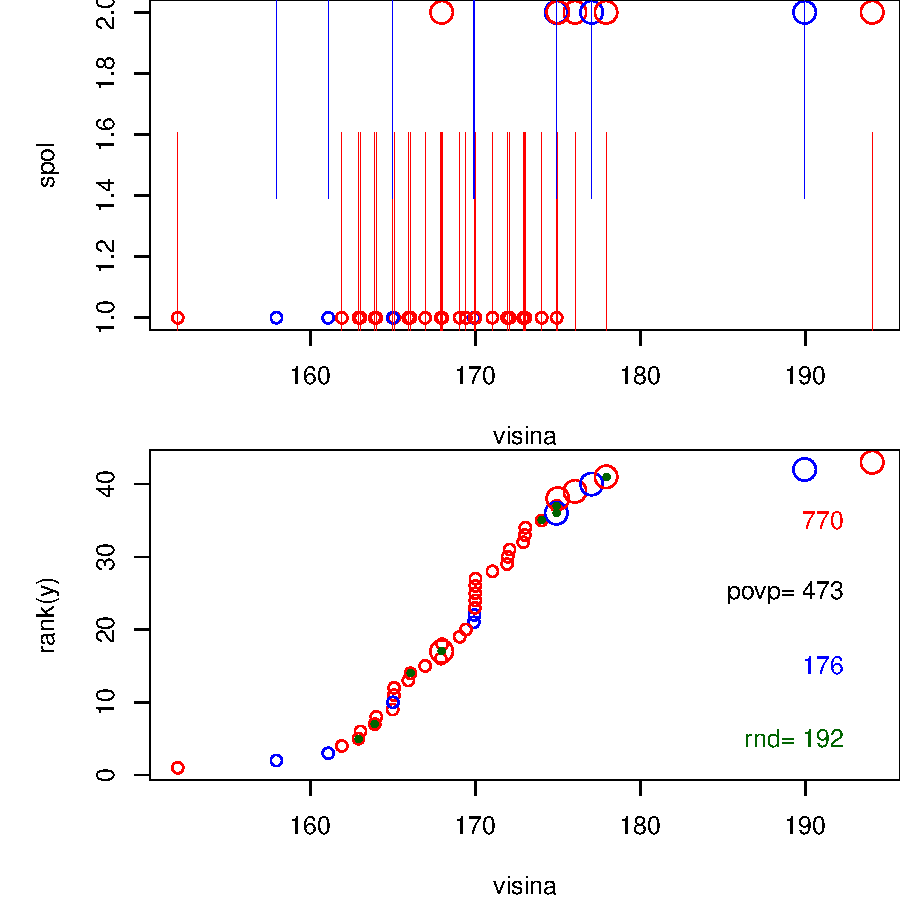
\includegraphics{./figs/SwPres-044}
\end{frame}
%% <<<<<<---------------------|


%% |--------------------->>>>>>
\begin{frame}[fragile]
\frametitle{Wilcoxon test v R}
\begin{Schunk}
\begin{Sinput}
> wilcox.test(jitter(visina) ~ spol)
\end{Sinput}
\begin{Soutput}
	Wilcoxon rank sum test

data:  jitter(visina) by spol 
W = 19, p-value = 2.296e-05
alternative hypothesis: true location shift is not equal to 0 
\end{Soutput}
\end{Schunk}

\end{frame}
%% <<<<<<---------------------|


\clearpage
\section{Kontingenca}

%% |--------------------->>>>>>
\begin{frame}[fragile]
\frametitle{Barva las in o�i}
\begin{Schunk}
\begin{Sinput}
> f <- table(lasje, oci)
> f
\end{Sinput}
\begin{Soutput}
        oci
lasje    svetle temne
  svetli     14     3
  temni      10    16
\end{Soutput}
\begin{Sinput}
> addmargins(f)
\end{Sinput}
\begin{Soutput}
        oci
lasje    svetle temne Sum
  svetli     14     3  17
  temni      10    16  26
  Sum        24    19  43
\end{Soutput}
\end{Schunk}
\end{frame}
%% <<<<<<---------------------|

%% |--------------------->>>>>>
\begin{frame}[fragile]
\frametitle{Pri�akovane frekvence}
\begin{Schunk}
\begin{Sinput}
> e <- outer(rowSums(f), colSums(f))/sum(f)
> addmargins(e)
\end{Sinput}
\begin{Soutput}
          svetle     temne Sum
svetli  9.488372  7.511628  17
temni  14.511628 11.488372  26
Sum    24.000000 19.000000  43
\end{Soutput}
\end{Schunk}
\end{frame}
%% <<<<<<---------------------|

\begin{frame}[fragile]
\frametitle{Razlika opa�enega in pri�akovanega}
\begin{Schunk}
\begin{Sinput}
> f - e
\end{Sinput}
\begin{Soutput}
        oci
lasje       svetle     temne
  svetli  4.511628 -4.511628
  temni  -4.511628  4.511628
\end{Soutput}
\begin{Sinput}
> (f - e)^2/e
\end{Sinput}
\begin{Soutput}
        oci
lasje      svetle    temne
  svetli 2.145235 2.709770
  temni  1.402654 1.771773
\end{Soutput}
\begin{Sinput}
> 1.96^2
\end{Sinput}
\begin{Soutput}
[1] 3.8416
\end{Soutput}
\end{Schunk}
\end{frame}

%% |--------------------->>>>>>
\begin{frame}[fragile]
\frametitle{Test $\chi^2$}
\begin{Schunk}
\begin{Sinput}
> alpha <- 0.05
> (df <- (ncol(f) - 1) * (nrow(f) - 1))
\end{Sinput}
\begin{Soutput}
[1] 1
\end{Soutput}
\begin{Sinput}
> (X2.krit <- qchisq(1 - alpha, df))
\end{Sinput}
\begin{Soutput}
[1] 3.841459
\end{Soutput}
\begin{Sinput}
> (X2 <- sum((f - e)^2/e))
\end{Sinput}
\begin{Soutput}
[1] 8.029432
\end{Soutput}
\begin{Sinput}
> (p <- 1 - pchisq(X2, df))
\end{Sinput}
\begin{Soutput}
[1] 0.004602328
\end{Soutput}
\begin{Sinput}
> if (X2 < X2.krit) cat("Spremenljivki NISTA odvisni (p =", 
+     round(p, 4), ").\n") else cat("Spremenljivki STA odvisni (p <", 
+     alpha, ") (p =", round(p, 4), ").\n")
\end{Sinput}
\begin{Soutput}
Spremenljivki STA odvisni (p < 0.05 ) (p = 0.0046 ).
\end{Soutput}
\end{Schunk}
\end{frame}
%% <<<<<<---------------------|

%% |--------------------->>>>>>
\begin{frame}[fragile]
\frametitle{Funkcija za test v R}
\begin{Schunk}
\begin{Sinput}
> chisq.test(lasje, oci, correct = FALSE)
\end{Sinput}
\begin{Soutput}
	Pearson's Chi-squared test

data:  lasje and oci 
X-squared = 8.0294, df = 1, p-value =
0.004602
\end{Soutput}
\end{Schunk}
\end{frame}
%% <<<<<<---------------------|

\subsection{Asociacija ( $2 \times 2$ )}

%% |--------------------->>>>>>
\begin{frame}[fragile]
\frametitle{Barva las in o�i}
\begin{Schunk}
\begin{Soutput}
        oci
lasje    svetle temne Sum
  svetli     14     3  17
  temni      10    16  26
  Sum        24    19  43
\end{Soutput}
\end{Schunk}
Asociacija ( $2 \times 2$ )

$$\frac{N(ad-bc)^2}{(a+b)(c+d)(a+c)(b+d)}$$
\begin{Schunk}
\begin{Sinput}
> sum(f) * det(matrix(f, 2, 2))^2/prod(colSums(f), 
+     rowSums(f))
\end{Sinput}
\begin{Soutput}
[1] 8.029432
\end{Soutput}
\end{Schunk}
\end{frame}
%% <<<<<<---------------------|

%% |--------------------->>>>>>
\begin{frame}[fragile]
\frametitle{Slika}
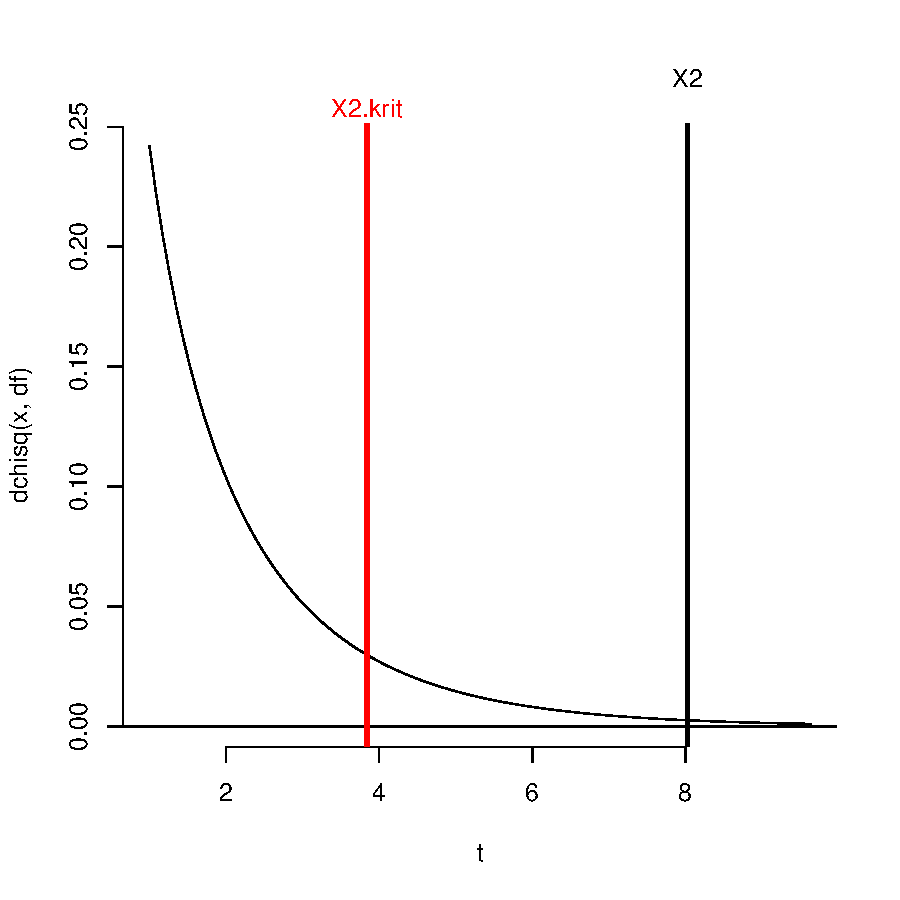
\includegraphics{./figs/SwPres-053}
\end{frame}
%% <<<<<<---------------------|
\clearpage
\section{Korelacija in regresija}

Slika Lenoarda da Vincija 'Virtruvian man' prikazuje razmerja razli�nih delov telesa. Vi�ina �loveka in
razpon rok naj bi bila pribli�no enaka. �e trditev dr�i, bi morale to�ke dolo�ene z vi�ino ($x$)
 in razponom rok ($y$) le�ati na premici $y=x$.

%% |--------------------->>>>>>
\begin{frame}[fragile]
\frametitle{Virtruvian man: Roke = Vi�ina}
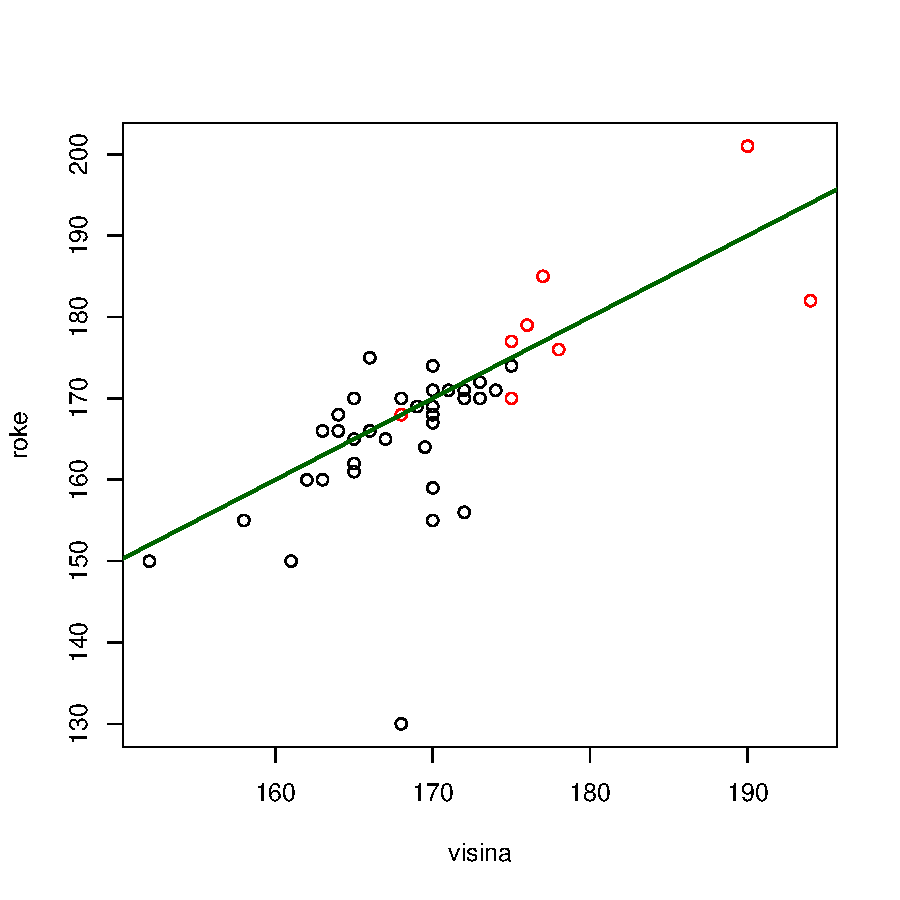
\includegraphics{./figs/SwPres-054}
\end{frame}
%% <<<<<<---------------------|

%% |--------------------->>>>>>
\begin{frame}[fragile]
\frametitle{Spremenljivke}
\begin{Schunk}
\begin{Sinput}
> select <- roke > 0
> x <- visina[select]
> y <- roke[select]
> spol <- spol[select]
> n <- length(x)
\end{Sinput}
\end{Schunk}
\end{frame}
%% <<<<<<---------------------|
%% |--------------------->>>>>>
\begin{frame}[fragile]
\frametitle{Osnovni ra�un}
\vspace{-1cm}
\begin{Schunk}
\begin{Sinput}
> (xbar <- mean(x))
\end{Sinput}
\begin{Soutput}
[1] 169.7326
\end{Soutput}
\begin{Sinput}
> (ybar <- mean(y))
\end{Sinput}
\begin{Soutput}
[1] 167.4419
\end{Soutput}
\begin{Sinput}
> sum((x - xbar) * (y - ybar))/(n - 1)
\end{Sinput}
\begin{Soutput}
[1] 54.1567
\end{Soutput}
\begin{Sinput}
> cov(x, y)
\end{Sinput}
\begin{Soutput}
[1] 54.1567
\end{Soutput}
\begin{Sinput}
> (r <- cov(x, y)/(sd(x) * sd(y)))
\end{Sinput}
\begin{Soutput}
[1] 0.6906298
\end{Soutput}
\begin{Sinput}
> r^2
\end{Sinput}
\begin{Soutput}
[1] 0.4769695
\end{Soutput}
\begin{Sinput}
> (b <- cov(x, y)/var(x))
\end{Sinput}
\begin{Soutput}
[1] 1.038539
\end{Soutput}
\begin{Sinput}
> (a <- mean(y) - b * mean(x))
\end{Sinput}
\begin{Soutput}
[1] -8.832009
\end{Soutput}
\end{Schunk}
\end{frame}
%% <<<<<<---------------------|




%% |--------------------->>>>>>
\begin{frame}[fragile]
\frametitle{Virtruvian man: Roke = Vi�ina}
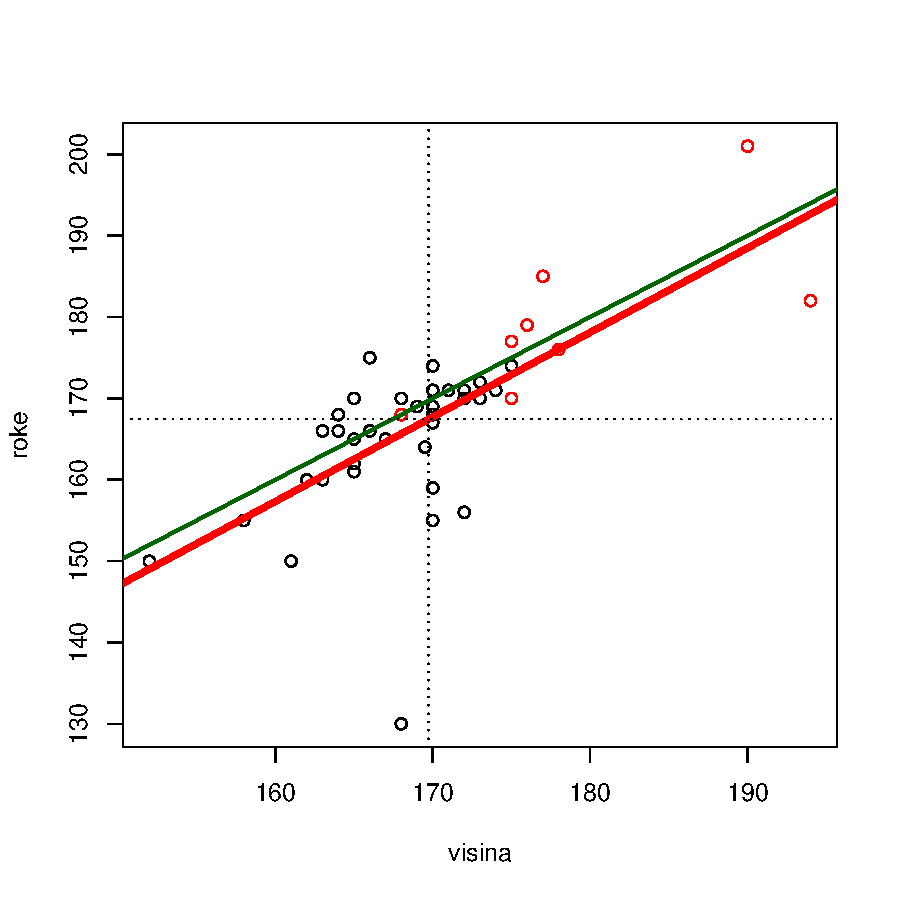
\includegraphics{./figs/SwPres-057}
\end{frame}
%% <<<<<<---------------------|

%% |--------------------->>>>>>
\begin{frame}[fragile]
\frametitle{Regresija v R}
\vspace{-1cm}
\begin{Schunk}
\begin{Sinput}
> cor(x, y)
\end{Sinput}
\begin{Soutput}
[1] 0.6906298
\end{Soutput}
\begin{Sinput}
> lsfit(x, y)$coefficients
\end{Sinput}
\begin{Soutput}
Intercept         X 
-8.832009  1.038539 
\end{Soutput}
\begin{Sinput}
> lm(y ~ x)$coefficients
\end{Sinput}
\begin{Soutput}
(Intercept)           x 
  -8.832009    1.038539 
\end{Soutput}
\begin{Sinput}
> lm(y ~ x * spol)
\end{Sinput}
\begin{Soutput}
Call:
lm(formula = y ~ x * spol)

Coefficients:
(Intercept)            x    spolmoski  
  20.648518     0.859143     4.642732  
x:spolmoski  
   0.003153  
\end{Soutput}
\end{Schunk}
\end{frame}
%% <<<<<<---------------------|

%% |--------------------->>>>>>
\begin{frame}[fragile]
\frametitle{Virtruvian man: Roke = Vi�ina}
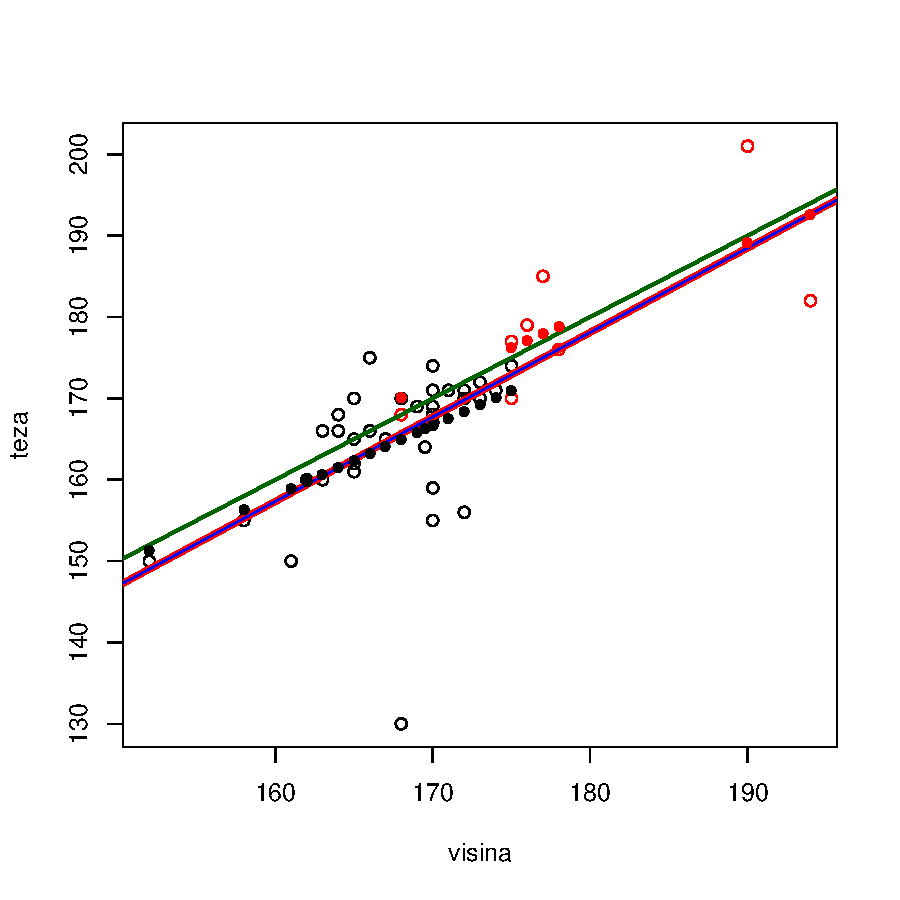
\includegraphics{./figs/SwPres-059}
\end{frame}
%% <<<<<<---------------------|

%% |--------------------->>>>>>
\begin{frame}[fragile]
\frametitle{Analiza variance za linearni model}
\begin{Schunk}
\begin{Sinput}
> anova(lm(roke ~ visina * spol))
\end{Sinput}
\begin{Soutput}
Analysis of Variance Table

Response: roke
            Df Sum Sq Mean Sq   F value    Pr(>F)
visina       1 2362.2  2362.2   37.0845 3.887e-07
spol         1  106.1   106.1    1.6657    0.2044
visina:spol  1    0.0     0.0 4.902e-05    0.9944
Residuals   39 2484.3    63.7                    
               
visina      ***
spol           
visina:spol    
Residuals      
---
Signif. codes:  0 '***' 0.001 '**' 0.01 '*' 0.05 '.' 0.1 ' ' 1 
\end{Soutput}
\end{Schunk}
\end{frame}
%% <<<<<<---------------------|


%% |--------------------->>>>>>
\begin{frame}[fragile]
\frametitle{Primerjava z vi�ino matere}
\vspace{-1cm}
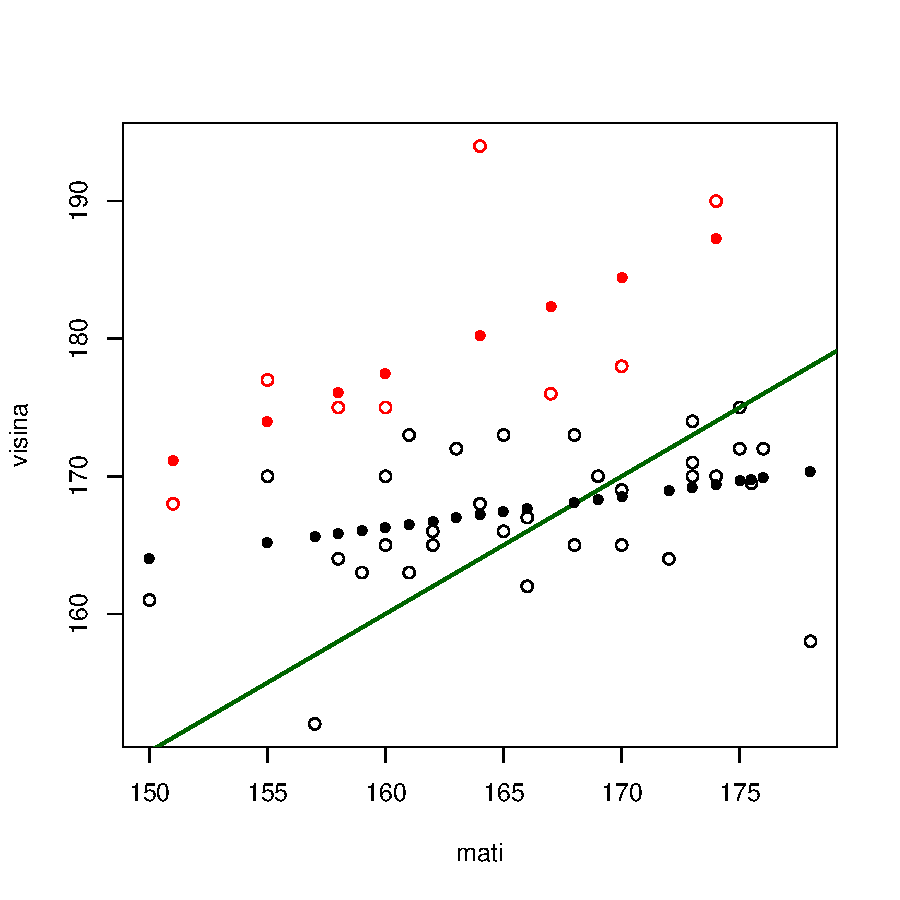
\includegraphics{./figs/SwPres-061}
\end{frame}
%% <<<<<<---------------------|

%% |--------------------->>>>>>
\begin{frame}[fragile]
\frametitle{Primerjava z vi�ino o�etov}
\vspace{-1cm}
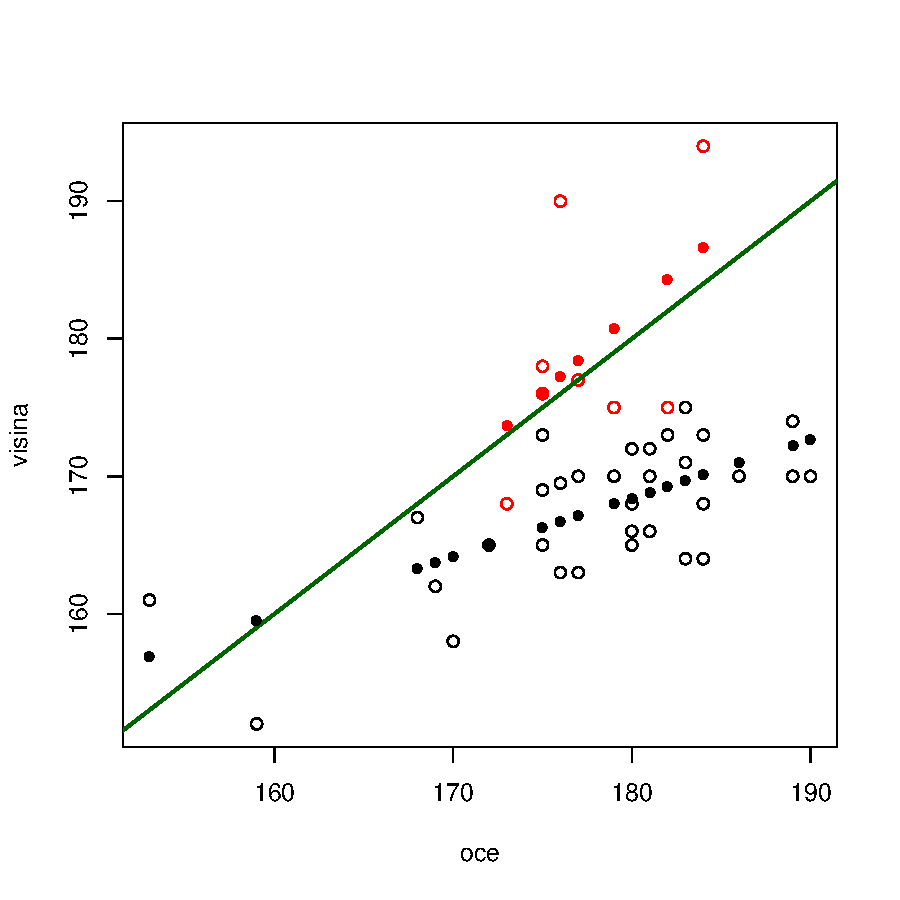
\includegraphics{./figs/SwPres-062}
\end{frame}
%% <<<<<<---------------------|

%% |--------------------->>>>>>
\begin{frame}[fragile]
\frametitle{Primerjava vi�in o�etov in mam}
\vspace{-1cm}
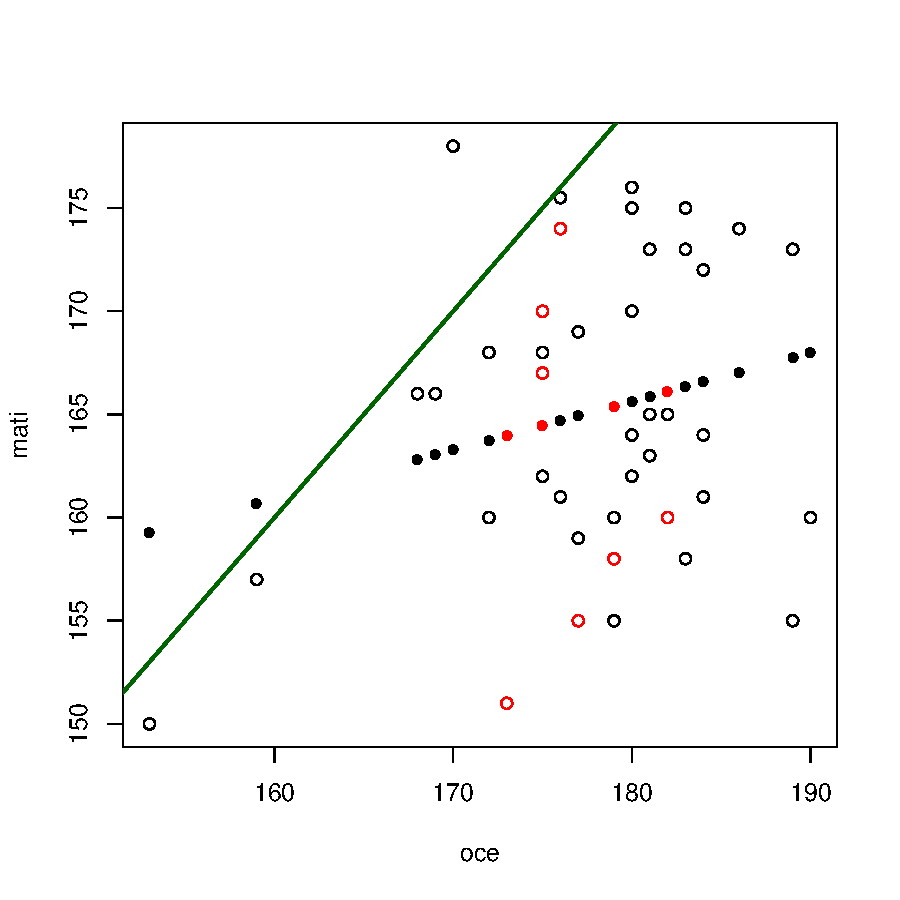
\includegraphics{./figs/SwPres-063}
\end{frame}
%% <<<<<<---------------------|


% ----------------------------------------------------------------
\bibliographystyle{amsplain}
\bibliography{ab-general}
\end{document}
% ----------------------------------------------------------------

